\documentclass{../template/Report}%方括号内写yuxi即生成预习报告\documentclass[yuxi]{../template/Report}
\settemplatedir{../template/}%设置模板路径

\exname{} %实验名称
\extable{} %实验桌号
\instructor{} %指导教师
\class{} %班级
\name{} %姓名
\stuid{} %学号

\nyear{} %年
\nmonth{} %月
\nday{} %日
\nweekday{} %星期几，e.g. \nweekday{三}
\daypart{}%上午/下午

\redate{} %如有实验补做，补做日期
\resitu{} %情况说明：

\begin{document}
\maketitle%输出封面

\section{预习报告（10分）}

\subsection{实验综述（5分）}
本实验利用非平衡直流电桥测量铜电阻的温度系数。实验原理基于惠斯通电桥的非平衡输出特性：当负载开路（$R_g \to \infty$）时，电桥输出电压 $U_g$ 能灵敏反映桥臂电阻的微小变化。

\begin{figure}[H]
    \centering
    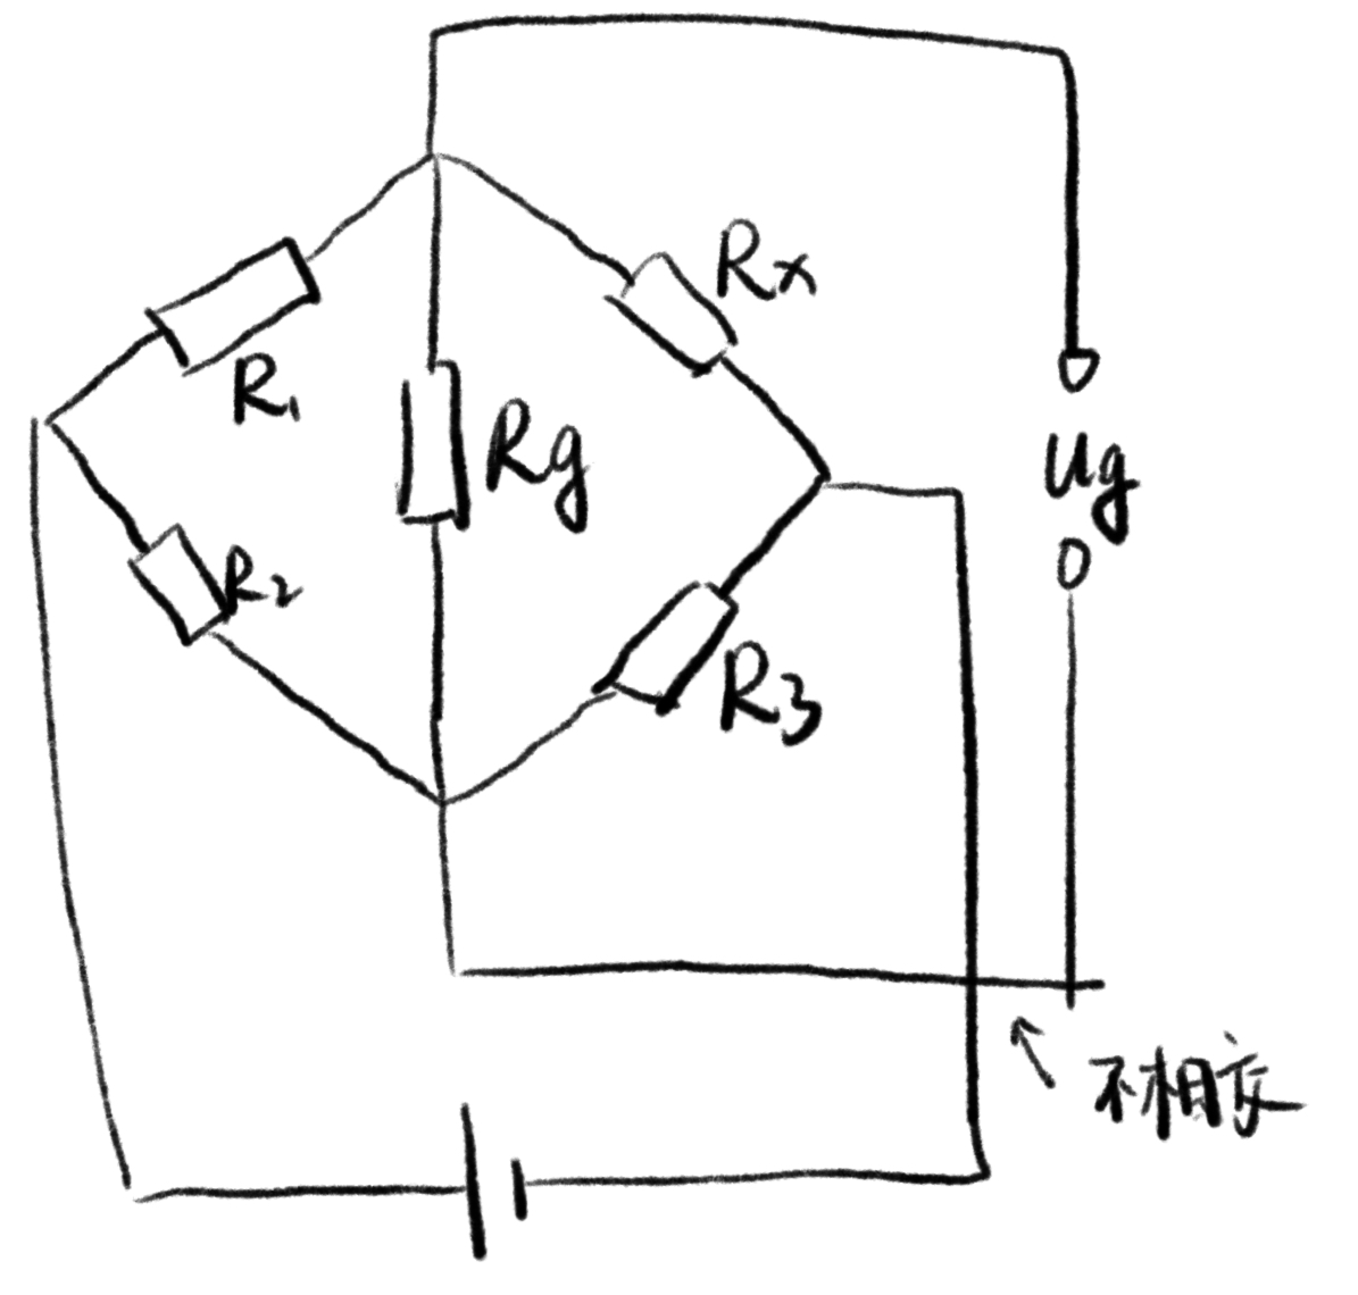
\includegraphics[width=0.6\textwidth]{./figure/2/非平衡电桥示意图.pdf}
    \caption{非平衡电桥原理图}
\end{figure}

在测量原理上，首先建立非平衡电桥的输出电压模型。根据分压原理，B、D两点间的电势差 $U_g$ 为：
\begin{equation}
    U_g = U_{BD} = \frac{R_2 R_x - R_1 R_3}{(R_1+R_x)(R_2+R_3)}\mathcal{E}
\end{equation}
实验中采用对称电桥配置，设定 $R_1=R_2=R_3=R_0$（取 $0^{\circ}\mathrm{C}$ 时的阻值），并将待测电阻 $R_x$ 视为随温度线性变化的函数 $R_x = R_t = R_0(1+\alpha t)$。将上述条件代入式(1)进行推导：
\begin{equation}
    U_g = \frac{R_0 \cdot R_0(1+\alpha t) - R_0 \cdot R_0}{(R_0 + R_0(1+\alpha t))(R_0 + R_0)}\mathcal{E}
\end{equation}
整理后消去 $R_0$，得到输出电压与温度 $t$ 的函数关系：
\begin{equation}
    U_g = \frac{\alpha t}{4+2\alpha t}\mathcal{E}
\end{equation}
由此式通过代数变换解出 $\alpha$，即为本实验的数据处理核心公式：
\begin{equation}
    \alpha = \frac{4U_g}{t(\mathcal{E} - 2U_g)}
\end{equation}
实验方法为：搭建电路并预调平衡，利用温控装置改变温度，记录不同温度点 $t$ 下的非平衡电压 $U_g$，代入上述公式计算 $\alpha$。

\subsection{实验重点（3分）}
\begin{enumerate}
    \item \textbf{理解测量原理}：掌握非平衡电桥如何将电阻的微小变化转化为电压信号，特别是特定对称条件（$R_1=R_2=R_3=R_0$）下公式的推导过程。
    \item \textbf{掌握实验操作}：熟练进行电桥的预调平衡操作，以及在变温环境下同步记录温度与电压数据的流程。
    \item \textbf{数据处理能力}：能够根据非线性输出公式反解出电阻温度系数 $\alpha$。
\end{enumerate}

\subsection{实验难点（2分）}
\begin{enumerate}
    \item \textbf{热平衡的控制}：加热过程中存在热惯性，需等待温度传感器示数稳定，确保其真实反映铜电阻的内部温度，避免滞后误差。
    \item \textbf{微弱信号的提取}：非平衡电压信号较小，需精确调平电桥，并尽量消除导线电阻和接触电阻引入的系统误差。
\end{enumerate}

\begin{fullreportonly}
    \section{原始数据（20分）}
    （将有老师签名的“自备数据记录草稿纸”的扫描或手机拍摄图粘贴在下方，完整保留姓名，学号，教师签字和日期。）

    \section{结果与分析（60分）}

    \subsection{数据处理与结果（30分）}

    \subsubsection{非平衡电桥测温度系数数据处理}

    \begin{table}[H]
        \centering
        \caption{非平衡电桥测温度系数数据记录表}
        \label{tab:non_equilibrium}
        \begin{tabular}{cccc}
            \toprule
            次序 & 温度 $t / \si{\degreeCelsius}$ & 不平衡电压 $U_g / \si{\milli\volt}$ & 计算 $\alpha / (\SI{e-3}{\per\degreeCelsius})$ \\
            \midrule
            1  & 30.0                         & 39.2                           & 4.279                                        \\
            2  & 35.0                         & 45.6                           & 4.311                                        \\
            3  & 40.0                         & 52.1                           & 4.357                                        \\
            4  & 45.0                         & 58.0                           & 4.354                                        \\
            5  & 50.0                         & 63.5                           & 4.331                                        \\
            6  & 55.0                         & 69.1                           & 4.326                                        \\
            7  & 60.0                         & 74.1                           & 4.289                                        \\
            8  & 65.0                         & 79.7                           & 4.300                                        \\
            \bottomrule
        \end{tabular}
        \par\vspace{1mm}
        {\footnotesize * 注：实验条件 $E = \SI{1.3}{\volt}$，理论值 $\alpha_{0} = \SI{4.280e-3}{\per\degreeCelsius}$}
    \end{table}

    根据公式 $\alpha_i = \frac{4U_g}{t(E-2U_g)}$ 计算得到 8 个温度点的 $\alpha_i$，其平均值为：
    \begin{equation}
        \bar{\alpha} = \frac{1}{8}\sum_{i=1}^{8}\alpha_i = \SI{4.318e-3}{\per\degreeCelsius}
    \end{equation}

    \subsubsection{平衡电桥测温度特性数据处理}

    \begin{table}[H]
        \centering
        \caption{平衡电桥测温度特性数据记录表}
        \label{tab:equilibrium}
        \begin{tabular}{ccc}
            \toprule
            次序 & 温度 $t / \si{\degreeCelsius}$ & $R_t / \si{\ohm}$ \\
            \midrule
            1  & 29.5                         & 56.94             \\
            2  & 35.0                         & 57.91             \\
            3  & 40.0                         & 59.16             \\
            4  & 45.0                         & 60.20             \\
            5  & 50.0                         & 61.15             \\
            6  & 55.0                         & 62.24             \\
            7  & 60.0                         & 63.18             \\
            8  & 65.0                         & 64.53             \\
            \bottomrule
        \end{tabular}
        \par\vspace{1mm}
        {\footnotesize * 注：实验条件 $E = \SI{1.3}{\volt}$}
    \end{table}

    根据上表数据，使用Origin对 $R_t$ 与 $t$ 进行最小二乘线性拟合，模型为 $R(t) = a + bt$。
    根据拟合结果\cref{fig:linear_fit}所得参数，并依据有效数字规则修约如下：
    \begin{itemize}
        \item 截距：$a = \SI{50.52}{\ohm}$
        \item 斜率：$b = \SI{0.2135}{\ohm\per\degreeCelsius}$
        \item 决定系数：$R^2 = 0.9987$
    \end{itemize}

    进而求得电阻温度系数（保留四位有效数字）：
    \begin{equation}
        \alpha = \frac{b}{a} = \frac{0.2135}{50.52} = \SI{4.226e-3}{\per\degreeCelsius}
    \end{equation}

    \begin{figure}[H]
        \centering
        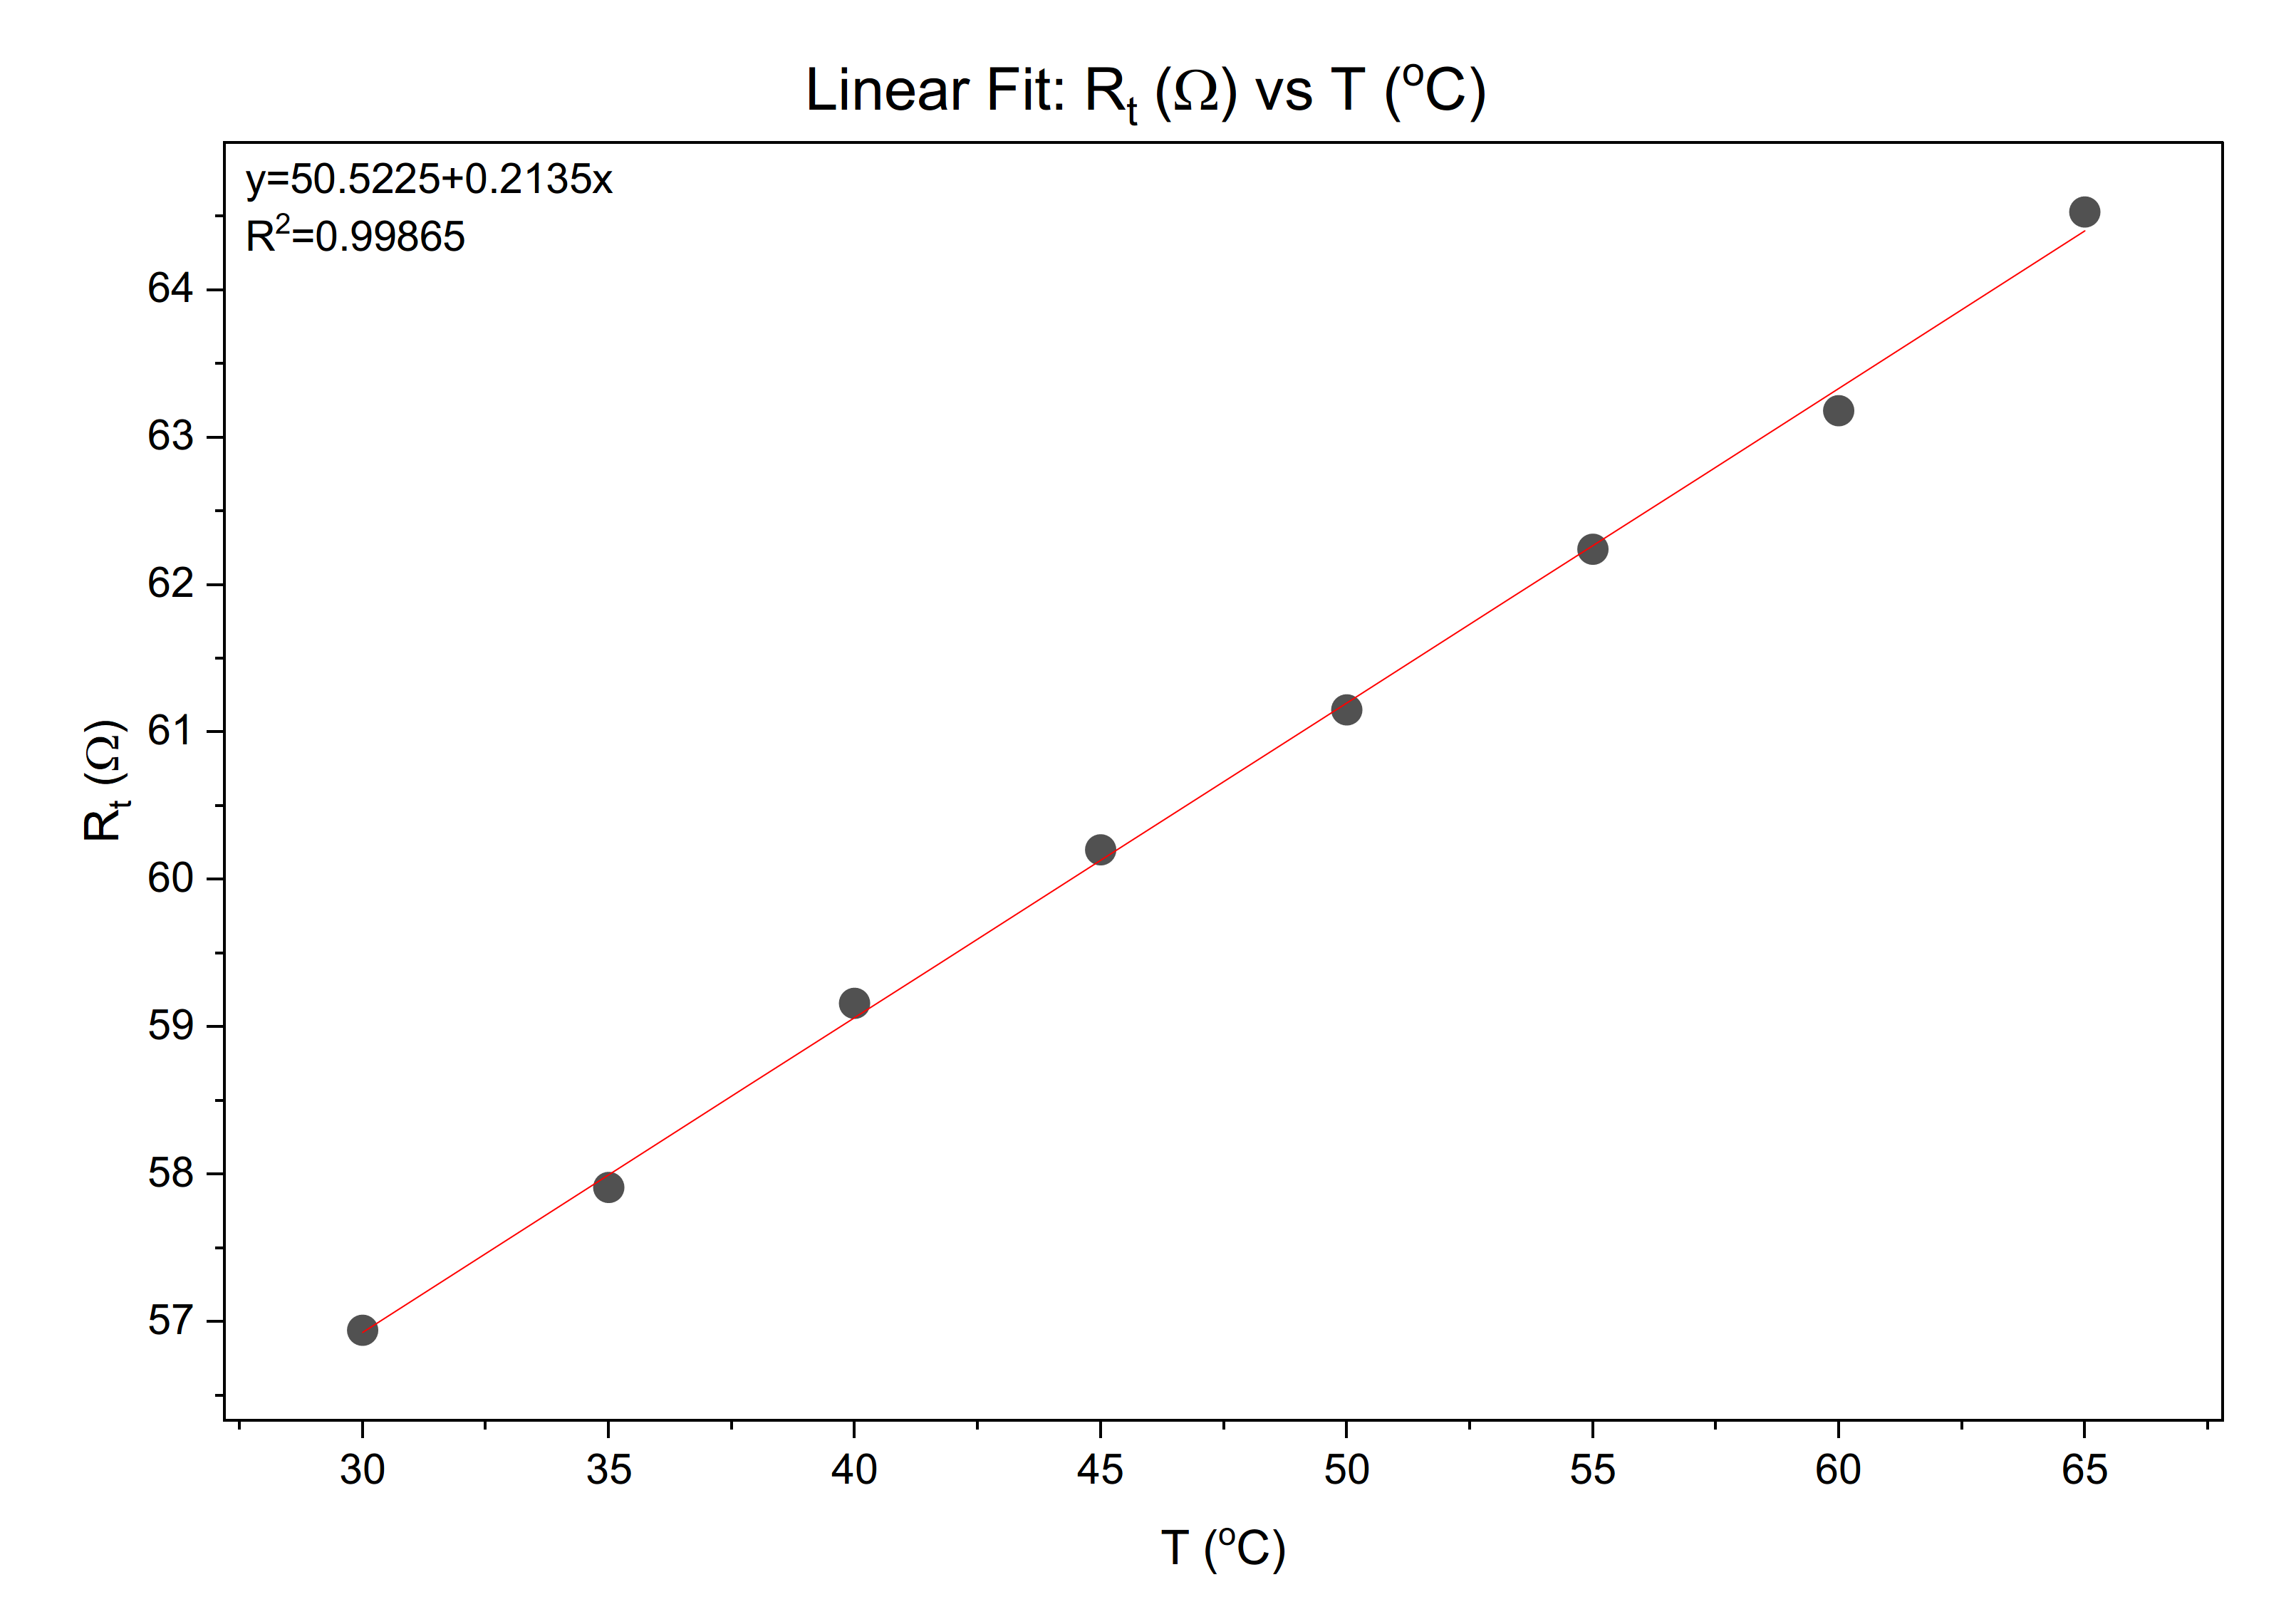
\includegraphics[width=0.7\textwidth]{./figure/2/fit.png}
        \caption{平衡电桥测温度特性拟合图}
        \label{fig:linear_fit}
    \end{figure}

    \subsection{误差分析（20分）}

    \subsubsection{非平衡电桥测量的统计与误差}
    对非平衡电桥所得 $\alpha_i$（单位 \si{\per\degreeCelsius}）：
    \begin{equation}
        \bar{\alpha} = \SI{4.318e-3}{\per\degreeCelsius}, \quad s = \SI{0.029e-3}{\per\degreeCelsius}
    \end{equation}

    计算 A 类不确定度：
    \begin{equation}
        u_A = \frac{s}{\sqrt{8}} = \SI{0.010e-3}{\per\degreeCelsius}
    \end{equation}

    结果：
    \begin{equation}
        \alpha_{\text{非平衡}} = (\num{4.318} \pm \num{0.010}) \times 10^{-3} \si{\per\degreeCelsius}
    \end{equation}

    与理论值 $\alpha_{0} = \SI{4.280e-3}{\per\degreeCelsius}$ 比较，相对偏差为：
    \begin{equation}
        E_1 = \frac{4.318 - 4.280}{4.280} \times 100\% \approx \SI{0.89}{\percent}
    \end{equation}

    \subsubsection{平衡电桥线性拟合误差分析}
    由最小二乘法线性拟合得到的温度系数为 $\alpha_{\text{平衡}} = \SI{4.226e-3}{\per\degreeCelsius}$。

    与理论值 $\alpha_{0} = \SI{4.280e-3}{\per\degreeCelsius}$ 比较，相对偏差为：
    \begin{equation}
        E_2 = \frac{\left|4.226 - 4.280\right|}{4.280} \times 100\% \approx \SI{1.26}{\percent}
    \end{equation}

    \subsection{结果讨论与误差分析}

    \subsubsection{结果验证}
    \begin{enumerate}
        \item \textbf{非平衡电桥法：} 测量结果略高于理论值（偏差约 \SI{0.89}{\percent}）。
        \item \textbf{平衡电桥法：} 测量结果略低于理论值（偏差约 \SI{1.26}{\percent}）。
        \item \textbf{综合误差分析：} 两种方法测得的铜电阻温度系数均与理论值吻合良好，相对误差均控制在 \SI{1.3}{\percent} 以内。且数据处理中有效数字保留合理，验证了本实验所采用测量方法及线性拟合手段的准确性。
    \end{enumerate}

    \subsubsection{误差来源分析}
    本实验虽然精度较高，但仍存在以下主要误差来源：
    \begin{enumerate}
        \item \textbf{温度测量与热滞后误差：} 实验加热过程中，铜电阻元件内部的温度变化可能滞后于仪器读出的温度。
        \item \textbf{电流热效应：} 测量过程中电桥电路接通，流经铜电阻的电流会产生焦耳热。这会导致电阻丝的实际温度略高于环境水温，从而使测得的电阻值偏大，引入系统误差。
        \item \textbf{电源电压的不稳定性：} 非平衡电桥法的计算公式 $\alpha \approx \frac{4U_g}{t(E-2U_g)}$ 强烈依赖于电源电动势 $E$。
              实验中假定 $E=\SI{1.3}{\volt}$ 恒定不变，但若电源内阻变化或电压波动，将直接影响 $U_g$ 的测量结果，进而影响 $\alpha$ 的计算。
        \item \textbf{仪器精度与读数误差：} 电阻箱的示值误差、数字万用表测量电压的精度限制，都会传递到最终结果中，造成误差。
    \end{enumerate}

    \subsection{实验探讨（10分）}
    （对实验内容、现象和过程的小结，不超过100字。）

    在本次实验，我成功验证了铜电阻的线性温度特性。
    通过实验，我了解了非平衡电桥的工作机理，明确了其输出电压与电阻变化量的函数关系，并熟悉了实验仪器的调节规范。

    在数据处理环节，通过对比平衡法与非平衡法的测量结果，我运用Origin等现代数据处理软件进行线性拟合，求取温度系数，
    并对误差来源进行了量化分析，从而对电桥测量电路的设计思想有了更直观的认识。

    \section{思考题（10分）}
    （解答教材或讲义或老师布置的思考题，请先写题干，再作答。）
    \subsection{简述非平衡电桥和平衡电桥之间的区别}
    \begin{enumerate}
        \item \textbf{测量原理的区别}
              \begin{itemize}
                  \item 平衡电桥采用“零值法”测量。
                        其核心原理是通过调节可变电阻臂，使电桥输出端的电位差趋于零，即中间的灵敏电流计读数为0，
                        利用电桥平衡公式计算被测电阻。
                        这种方法测量精度高，受电源波动影响小，但测量过程较慢，仅适用于静态测量。
                  \item 非平衡电桥采用“偏转法”测量。
                        其桥臂电阻通常固定，利用电桥偏离平衡状态时输出电压 $U_g$ 与被测电阻变化量 $\Delta R$ 之间的函数关系，
                        通过测量 $U_g$ 的大小来反推阻值变化。
              \end{itemize}
        \item \textbf{结构与功能的区别：}
              \begin{itemize}
                  \item 平衡电桥结构中必须包含可调的标准电阻，主要用于精确测量某一固定时刻的电阻绝对值。
                  \item 非平衡电桥通常与传感器配合使用，电路参数固定，
                        用于将电阻的变化实时转化为电压信号输出，适用于动态、连续的测量场景。
              \end{itemize}
    \end{enumerate}

    \subsection{非平衡电桥在工程中有哪些应用？请举例说明}
    非平衡电桥在工程中是传感器技术的核心电路结构之一，
    广泛用于将非电学量转换为电学量。具体的应用场景包括：

    \begin{enumerate}
        \item \textbf{电阻应变片传感器（测力/称重）：}
              在土木工程和电子称重中，将金属或半导体应变片接入非平衡电桥。
              当物体受力发生形变时，应变片的电阻发生微小变化，电桥将其转化为电压信号输出，从而测得压力、拉力或扭矩。
        \item \textbf{工业测温：}
              利用热敏电阻作为非平衡电桥的一个臂。
              当环境温度变化导致电阻改变时，电桥输出电压随之变化。
              该信号经放大后可用于数字温度计显示或空调、加热炉的自动闭环控制。
        \item \textbf{气体与压力检测：}
              在压阻式传感器中，利用硅膜片的压阻效应构成非平衡电桥，可用于汽车进气压力监测或血压计中，
              实现对微小气压变化的实时捕捉。
    \end{enumerate}
\end{fullreportonly}
\insertnotes
\end{document}